%%%%%%template by Daniel Parker
%%%%%%http://dug.math.brown.edu/
\documentclass[10pt,twoside]{article}
%%%%%%%%%packages%%%%%%%%%
\usepackage{amsmath}
\usepackage{amssymb}
\usepackage{amsfonts}
\usepackage{amsthm}
\usepackage{mathrsfs}
\usepackage{mathtools}
\usepackage{colonequals} 	
\usepackage{graphicx}
\usepackage{fancyhdr}
\usepackage{multirow}
\usepackage{siunitx}
\usepackage{tikz}
\usepackage[headings]{fullpage}

%%%%%%%%%header%%%%%%%%%
\pagestyle{fancy}
\fancyhead{} % clear all header fields
\renewcommand{\headrulewidth}{0.2pt}
\fancyhead[RO,LE]{\bfseries \hspace{1in}\rightOne\phantom{\hspace{1in}}\\ \hspace{1in}\rightTwo\hspace{1in}}
\fancyhead[RE,LO]{\bfseries \hspace{1in}\leftOne\phantom{\hspace{1in}}\\ \hspace{1in}\leftTwo\hspace{1in}}
\fancyhead[C]{\bfseries \centerOne\\\centerTwo}
\fancyfoot{}
\setlength{\voffset}{-1in+1.5em}
\fancyheadoffset{1in}
\addtolength{\textheight}{1in}

%%%%%%%%%theorem environment and numbering%%%%%%%%%
%%%%%%%%%uses amsthm package
\newtheorem{thm}{Theorem}
\newtheorem{prop}[thm]{Proposition}
\newtheorem{lm}[thm]{Lemma}
\newtheorem{defn}[thm]{Definition}
\newtheorem{rem}[thm]{Remark}
\newtheorem{cl}{Claim}[thm]
\newtheorem{cor}[thm]{Corollary}

\theoremstyle{definition}
\newtheorem{eg}[thm]{Example}

%%%%%%%%%exercise numbering%%%%%%%%%
\newtheoremstyle{exercise}{}{}{\itshape}{}{\bfseries}{:}{.5em}{\thmname{#1} \thmnumber{#2}\thmnote{(#3)}}
\theoremstyle{exercise}
\newtheorem{ex}{Exercise}
\newcommand{\nextex}[1]{\begin{ex}\end{ex}}
\newcommand{\nextexP}[1]{\begin{ex}#1\end{ex}}
\newcommand{\setex}[1]{\setcounter{ex}{#1-1}\begin{ex}\end{ex}}
\newcommand{\setexP}[2]{\setcounter{ex}{#1-1}\begin{ex}#2\end{ex}}

%%%%%%%%%notation shortcuts%%%%%%%%%
\newcommand{\R}{\mathbb{R}}
\newcommand{\Q}{\mathbb{Q}}
\newcommand{\Z}{\mathbb{Z}}
\newcommand{\N}{\mathbb{N}}
\newcommand{\F}{\mathbb{F}}
\newcommand{\C}{\mathbb{C}}


\newcommand{\n}[1]{\left| #1 \right|}%%adjustable-height norm shortcut
\newcommand{\set}[2]{\left\{#1\left|\; #2 \right. \right\}}%%set notation shortcut with a line
\newcommand{\setc}[2]{\left\{#1\; :\; #2 \right\}}%%set notation shortcut with a colon
\newcommand{\st}[1]{\left\{#1\right\}}%%set notation shortcut with no condition
\newcommand{\ce}{\colonequals}%%shortcut to write \colonequals

\newcommand{\bvi}{\hat{\mathbf{i}}} %basis vector i
\newcommand{\bvj}{\hat{\mathbf{j}}} %basis vector j
\newcommand{\bvk}{\hat{\mathbf{k}}} %basis vector k
\newcommand{\bvr}{\hat{\mathbf{r}}} %basis vector r
\newcommand{\bvt}{\hat{\mathbf{\theta}}}%basis vector theta
\newcommand{\bvx}{\hat{\mathbf{x}}} %basis vector x
\newcommand{\bvy}{\hat{\mathbf{y}}}%basis vector y
\renewcommand{\v}[1]{\mathbf #1}%%shortcut to make a vector N.B. this overwrites the default command for \v which makes a caret over the letter

\newcommand{\aut}{\operatorname{Aut}}
\newcommand{\mor}{\operatorname{Mor}}
\newcommand{\chr}{\operatorname{char}}
\newcommand{\spn}{\operatorname{span}}
\newcommand{\tr}{\operatorname{Tr}}
\newcommand{\im}{\operatorname{Im}}


%%%MODIFY THESE LINES TO CHANGE THE HEADER
\newcommand{\leftOne}{Brown University}
\newcommand{\leftTwo}{Prof. Dell'Antonio}
\newcommand{\centerOne}{Overview and Technical Description of \texttt{jedisim}}
\newcommand{\centerTwo}{26 July  2013}
\newcommand{\rightOne}{\thepage}
\newcommand{\rightTwo}{Dan Parker}

\begin{document}
\section{Purpose}

  Gravitational Lensing provides an accurate way to determine the mass distribution of objects based solely on the mass present, and is impartial to the details of how the mass interacts. Lensing is therefore ideal to study the mass distributions of galaxy clusters, which are often surrounded by dark matter halos. Moreover, since lensing is an independent measurement, it can be used to calibrate other measurement techniques such as x-ray emission or velocity dispersion measurements.  

  However, gravitational lensing measurements of mass distributions are subject to the same pitfalls as all observational science. Namely, it is tricky to determine the magnitude and sources of errors in measurement. If there were a ``perfect'' galaxy cluster whose mass distribution was known exactly, then it would be easy to quantify errors in the lensing measurement by comparing to that standard. Of course, no such ``perfect'' clusters exist. Therefore, the best alternative is to \textit{simulate} a ``perfect'' cluster and use it to determine and minimize errors.

  Any simulation is only as accurate as the model and parameters used to create it. Indeed, systemic inaccuracies in error measurements are inevitably introduced by whatever differences exist between the simulation and actual galaxy clusters. The best way to counteract this and reduce inaccuracies is to make the model and its parameters as physically accurate as possible. This, in turn, is limited by the computational power available and the precision of the parameters used to calibrate the model. Judicious selection of what approximations and simplifications are used is required to make the model. This report details and explains the \texttt{jedisim} model and its parameters.


\section{Overview}
The \texttt{jedisim} simulation models the effect of a foreground galaxy cluster on the shapes of background galaxies. Broadly, there are three main components of the simulation:
\begin{enumerate}
  \item Making the field of background galaxies.
  \item Distorting the light from the background galaxies in accordance with a specified mass distribution.
  \item Accounting for the blurring and distortion of the light imposed by Earth's atmosphere and optical properties of the telescope.
\end{enumerate}
The three steps are performed as independently as possible so that the model can be improved in a modular fashion. An effort is made to simulate galaxies individually and not combine them into a single image as late as possible so that redshift-dependent effects can be included. The first two steps are performed at the resolution of the Hubble Space Telescope (0.03 arcseconds per pixel) with an image size of 40960 by 40960 pixels In the final step, images are created as they would be observed by the upcoming LSST telescope.

\section{Simulating A Galaxy Field}
The background galaxy field is simulated one galaxy at a time. 


The shape of each galaxy is taken from a HST UDF image where individual galaxies are cut out and made into ``postage stamps'' so that a galaxy appears alone on a black background of size 600 by 600--- see Figure \ref{fig:postage_stamp}. The sample of 128 postage stamps is large enough that there is a fairly diverse set of galaxy shapes and orientations.

\begin{figure}
  \begin{center}
    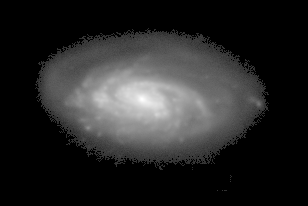
\includegraphics[scale=10]{images/example_galaxy.png}
  \end{center}
  \caption{An example ``postage stamp'' galaxy.}
  \label{fig:postage_stamp}
\end{figure}


Galaxies are simulated from 22\textsuperscript{nd} to 28\textsuperscript{th} magnitude, inclusive. Based on [cite whatever paper we found this in] a density of $1.242 \times 10^6$ galaxies per square degree is used, translating to 138,000 galaxies for one 40,960 by 40,960 image. This value is chosen with the expectation that a significant portion of these galaxies, especially at higher magnitudes, will be both faint and broad and will thus fall below the noise level or otherwise appear too faint to actually distinguish as galaxies, adding a realistic cosmic light background to the images. For each galaxy, several parameters are selected in a specific order:

\begin{description}
  \item[Magnitude] The magnitude of each galaxy is selected between 22\textsuperscript{nd} to 28\textsuperscript{th} magnitude with the distribution given by the power law
    \begin{equation}
      P(M) = \exp\left( A\log_{10}M \right)
      \label{eq:mag_power_law}
    \end{equation}
    where $M$ is the magnitude and $A = 0.33$ is a physically realistic constant.[cite where this value came from] The magnitude zero-point is taken to be 30 throughout the simulations by convention.

  \item[Radius] The database of r50 galaxy radii from [cite where the radii database came from] is used to select galaxy radii. Specifically, the database is binned by integer magnitude number, and a list of radii is made for each magnitude. Since each galaxy is already assigned a magnitude, it has a corresponding bin, and an r50 radius is chosen randomly from that bin.

  \item[Image] A postage stamp image is chosen at random from the postage stamps whose r50 value is larger than the r50 assigned to the galaxy. This is done so that images are always sized down.

  \item[Redshift] The database of galaxy redshift from [cite wherever it came from] is used and, as with radius, binned by integer magnitude. For each galaxy, a redshift is selected from the corresponding magnitude bin. Alternatively, a single redshift (i.e. z=1.5) can be chosen for all galaxies.

  \item[Position] The center of the postage stamp is selected as a pair of uniformly distributed floating points (for $x$ and $y$ position) from the range $[301, 40660]$. This range is taken to ensure that the entire image lies completely within the range $[0,40960]$. Eventually, a border of size $480$ will be trimmed from each side of the image, ensuring a uniform distribution of galaxy positions with no edge effects.

  \item[Angle] An angle is chosen uniformly in the range $[0,360)$ through which the postage stamp will be rotated. This is to ensure the orientation of the galaxies is random. The orientation of galaxies has at least three degrees of freedom, but since we are dealing with 2D projections of galaxies, we can only make the orientation random in one degree of freedom, with some additional variability coming from the diverse orientations of the postage stamps. 
\end{description}

Once these parameters are chosen for each galaxy, an image is made which satisfies those parameters. Specifically, the source postage stamp is used as a base, then photo-scaled to the correct magnitude, and scaled down to the correct r50 radius and rotated through the assigned angle using a bilinear interpolation. The galaxy is then cut out, so that the image consists of the smallest rectangle that contains all non-zero pixels of the galaxy. Each transformed postage stamp galaxy is saved as a FITS image. A list is made of all the galaxies with all the parameters which are not inherent to the image including redshift, size of the postage stamp, and place in the large 40,960 by 40,960 image where the lower left corner of the transformed postage stamp should be embedded.

We now have all the information for the background image: an accurate number of galaxies at well-distributed sizes, magnitudes, orientations, positions and (optionally) redshifts. The distributions are as close to realistic as possible and the image greatly resembles a HST UDF image.

\section{Simulating Gravitational Lensing}
The next step in the simulation is to emulate the effects of gravitational lensing caused by a galaxy cluster. In the weak field limit, for a point mass, this is governed by the Lens Equation
\begin{equation}
  \vec{\beta} = \vec{\theta} - \vec{\alpha}(\vec{\theta}) = \vec{\theta} - \frac{D_{ls}}{D_s}\vec{\hat{\alpha}}(\vec{\theta})
  \label{eq:lensing}
\end{equation}
where $\vec{\beta}$ is the angle between the light source and the point mass, $\vec{\theta}$ is the angle between the point mass and the apparent position of the light source, $\vec{\alpha}(\vec{\theta})$ is the deflection angle of the light at $\vec{\theta}$, $\vec{\hat{\alpha}}(\vec{\theta})$ is the corresponding unit vector, and $D_{ls}$ and $D_s$ are the angular diameter distance from the lens to the source and the observer to the source respectively. The deflection $\vec{\hat{\alpha}}$ is a vector quantity and (in the weak field limit), the deflections from a distribution of mass add linearly.


For computational simplicity, the gravitational lens is specified as a radially symmetric mass distribution with the center at an arbitrary location and arbitrary redshift. The radial distribution can be one of two profiles:
\begin{description}
  \item[Singular Isothermal Sphere] This Singular Isothermal Sphere (SIS) profile is the simplest model of a galaxy cluster, and is a good first approximation. It's density is given by
    \begin{equation}
      \rho(r; \sigma_v) = \frac{\sigma_v^2}{2\pi Gr^2}
      \label{eq:SIS_density}
    \end{equation}
    where $\sigma_v$ is the velocity dispersion and $G$ is the universal gravitational constant. This profile has the awkward properties that the total mass diverges for $r \to \infty$. Ignoring this, it is still a reasonable approximation close to the cluster. The deflection due to an SIS profile is given by 
    \begin{equation}
      \frac{\alpha(r; \sigma_v)}{r} = \frac{4\pi}{r}\left( \frac{\sigma_V}{c} \right)^2 \frac{\text{pixel scale}}{3600}\frac{\pi}{180}
      \label{eq:SIS_deflection}
    \end{equation}
    where $r$ is the radius in pixels, $\sigma_v$ is the dispersion parameter in km/s, $c$ is the speed of light in km/s, and $\text{pixel scale} = 0.03$ is the resolution of the image in arcseconds per pixel.

  \item[Navarro-Frenk-White Profile] The Navarro-Frenk-White (NFW) profile is one of the most accurate models of the mass distribution of clusters. It made discovered to emperically fit $n$-body simulations of clusters quite well and has had success fitting actual clusters as well.
    The NFW profile can be expressed in several different ways depending on what parameters are used. Using the critical density $\rho_0$ and the scale radius $R_s$, the density of the NFW profile is given by
    \begin{equation}
      \rho(r) = \frac{\rho_0}{\frac{r}{R_s}\left( 1+\frac{r}{R_s} \right)^2}
      \label{eq:NFW_density}
    \end{equation}

    The deflection in pixels by the NFW profile is given by
    \begin{align}
      \nonumber
      \frac{\alpha(r; M_{200}, c)}{r} \ &=  \frac{4GM_{200}\delta'_c}{9\times 10^5 D_L\, r\, \theta }\frac{\text{pixel scale}}{3600}\frac{\pi}{180}\\
      \ & \quad \times\
\left[\log \frac{x}{2} +  
      \begin{cases}
        \frac{2}{\sqrt{1-x^2}}\operatorname{arctanh}\left( \sqrt{\frac{1-x}{1+x}} \right) & \text{ if $x \in (0, 1)$}\\
        1 & \text{ if $x=1$}\\
        \frac{2}{\sqrt{x^2-1}}\arctan\left( \sqrt{\frac{x-1}{1+x}} \right) & \text{ if $x > 1$.}\\
      \end{cases}
      \right]
      \label{eq:NFW_deflection}
    \end{align}
    where $r$ is the radius in pixels, $M_{200}$ is the virial radius, $c$ is \textit{not} the speed of light, but rather a unitless concentration parameter for the NFW profile, $G$ is the universal gravitational constant with value $G = 4.302$ in these units, $D_L$ is the angular diameter distance of the cluster for a given cosmology, $\delta'_c$ is a modified version of the standard $\delta_c$ constant for the NFW profile 
    \[
      \delta'_c = \frac{1}{\log(1+c)-\frac{c}{1+c}},
    \]
    theta is the radius in radians 
    \[
      \theta = \frac{\text{pixel scale}}{3600}\frac{\pi}{180} r,
    \]
    and lastly $x$ is a unitless variable given by
    \[
      x = \frac{c D_L}{10.0}\left(\frac{G}{H_0^2}\right)^{-1/3}\theta
    \]
    where $H_0$ is the Hubble constant at the present time, and $c$ is again the concentration parameter.
\end{description}

\texttt{jedisim} permits an arbitrary number of lenses whose type (SIS or NFW), center point, redshift, and profile parameters are all specified by a configuration file. At this point, the redshift of all lenses must be the same. The deflection at an arbitrary point is the superposition of the deflections from all the lenses. The task is then to determine how this deflection changes the image of each galaxy.

Consider the universe as three parallel planes: the source plane where the background galaxies lie, the lens plane where the mass distribution lies, and the observation plane which is near earth but above the atmosphere. The light from the source plane going towards Earth will go through the lens plane and get deflected, and will form a distorted image of the source plane on the observation plane. The nature of the lensing equation is such that, given a point on the observation plane, and the mass distribution on the lens plane (or equivalently, the deflection function on the lens plane), you can say what point on the source plane light will come from. However, it is not possible to go backwards: given a point on the source plane, it is difficult to say where the light will go. 

In this simulation, all three planes are grids made of pixels. The area of the sky under consideration is small enough that we can treat all pixels as squares. The source plane is the (virtual) image created by the first part of the simulation --- i.e. a scalar-valued function $\text{Intensity}(x,y)$, the lens plane has the vector-valued deflection function $\vec{\hat{\alpha}}(x,y)$ and we want to compute the intensity function of the observation plane. Concretely, let $I_s(x,y)$ and $I_o(x,y)$ be the intensity functions of the source and observation planes respectively and let $\vec{\hat{\alpha}}(x,y)$ be the deflection function. Of course, $I_s(x,y)$ and $I_o(x,y)$ are only defined when $x$ and $y$ are integers. From then lensing equation, we then have
\begin{equation}
  I_o(x,y) = I_s\left(\operatorname{round}\left((x,y) - \frac{D_{ls}}{D_s}\vec{\hat{\alpha}}(x,y)\right) \right)
  \label{eq:discrete_lens}
\end{equation}
where $\operatorname{round}$ round the vector to the nearest integer-valued tuple. With large densities, $\vec{\hat{\alpha}}$ can change a lot over a single pixel. It is therefore useful to use \textit{subpixel} precision: we want to chop up each pixel into a grid and make its value the average of each of the subpixels. Letting $J_{o,4}(x,y)$ be the intensity of the observed image with subpixel size 4, we have
\begin{equation}
  J_{o,4}(x,y) = \frac{1}{4^2} \sum_{i=0}^3 \sum_{j=0}^3 I_s\left( \operatorname{round}\left( (x+i\delta, y+j\delta) - \frac{D_{ls}}{D_s}\vec{\hat{\alpha}}(x+i\delta, y+j\delta) \right) \right)
  \label{eq:discrete_lens_subpixel}
\end{equation}
where $\delta = 1/4$. 

In theory, this does it. We can loop over both $x$ and $y$ in the range $0$ to $40960$ and compute $J_{0,4}(x,y)$ for each one. However, $J_{o,4}$ depends on the distance to the source plane, which is different for every galaxy. Naively, this means that we would have to loop over every pixel in the grid for all 138,000 galaxies. This is an impractical number of computations. However, most of these computations are unnecessary. Each galaxy is tiny --- the image for each galaxys is never larger than 200 by 200 and usually about 30 by 30. Even with the most severe lensing, the image of each galaxy in the observation plane will only have a few thousand non-zero datapoints. If we knew \textit{a priori} where those pixels were, it would only be necessary to do a few thousand computations per galaxy instead of $40960^2$ computations. The only problem is we can only go backwards from the observation to the source plane, not the other way around because of the possibility of strong lensing effects where a pixel on the source plane is observed on two different observation pixels.

The solution is to approximate the subset of the observation plane where the galaxy will lie in such a way that the subset is never too small --- it always contains all non-zero pixels. It is useful to introduce the concept of an \textit{information box} of an image. Let the information box is the minimal rectangle which contains all non-zero pixels. An image can then be completely specified by the intensity of the image inside the box (which implicitly includes the box's width and height), and the location of any one of its corners, say the lower left. The galaxies in the source plane are already in this information box form. What we want to do is find the information box of their images on the observation plane.

To do this, superdivide the the observation plane into a coarser grid with $4096$ by $4096$ pixels to a grid square, making a $4096$-grid of size $10$ by $10$. For each coarse grid square, we want to compute the information box it can draw upon in the source plane. For a coarse grid square let $\text{B}(X,Y)$ be the $4$-tuple which gives the minimum and maximum of both components of $\vec{\hat{\alpha}}$ over that coarse grid square.
\begin{equation}
  \text{B}(X, Y) = \begin{bmatrix}
    \min\setc{\left[\vec{\hat{\alpha}}(x,y)\right]_x}{x \in [4096X, 4096(X+1)-1], y \in [4096Y, 4096(Y+1)-1]}\\[1em] 
    \max\setc{\left[\vec{\hat{\alpha}}(x,y)\right]_x}{x \in [4096X, 4096(X+1)-1], y \in [4096Y, 4096(Y+1)-1]}\\[1em]
    \min\setc{\left[\vec{\hat{\alpha}}(x,y)\right]_y}{x \in [4096X, 4096(X+1)-1], y \in [4096Y, 4096(Y+1)-1]}\\[1em] 
    \max\setc{\left[\vec{\hat{\alpha}}(x,y)\right]_y}{x \in [4096X, 4096(X+1)-1], y \in [4096Y, 4096(Y+1)-1]}\\[1em] 
    \end{bmatrix}.
  \label{eq:grid_alpha_box}
\end{equation}

Then, given a galaxy and its redshift (and hence $D_{ls}$ and $D_s$) and a coarse grid square, we can quickly determine the information box of the coarse grid square: which set of pixels in the source plain it can draw from in computing $J_{o,4}$. Namely, the $x$ and $y$ minima and maxima of this information box are given by
\begin{equation}
  \text{IB}(X,Y;D_{ls},D_s) = \begin{bmatrix}
    4096(X+1)-1-\frac{D_{ls}}{D_s}B(X,Y)_1\\
    4096X-\frac{D_{ls}}{D_s}B(X,Y)_2\\
    4096(Y+1)-1-\frac{D_{ls}}{D_s}B(X,Y)_3\\
    4096Y-\frac{D_{ls}}{D_s}B(X,Y)_4\\
  \end{bmatrix}
  \label{eq:grid_info_box}
\end{equation}
where $B(X,Y)_i$ represents the $i$\textsuperscript{th} component of $B(X,Y)$. Then for a specific galaxy, we can check if the box defined by $IB(X,Y; D_{ls}, D_s)$ intersects the information box of that galaxy in the source plane. If they do not intersect, then all the pixels inside the course grid square $(X,Y)$ must be zero. If they do intersect, then some may be non-zero and each pixel of $(X,Y)$ may need to be computed.

In practice, it is fastest to define several coarse grids. In this implementation, grids of size $4096$, $512$, $64$ and $8$ are used. The algorithm to determine what pixels to compute is as follows:
\begin{enumerate}
  \item Compute $B(X,Y)$ for each of the grid sizes.
  \item Loop over all galaxies.
  \item For each galaxy, loop over the largest grid. For each grid square, calculate the information bounding box of that grid square. If it intersects the information bounding box of the galaxy, then loop over all the grid square in the next-finest grid. Continue down until the grid of size $8$. If the information bounding box of the grid of size $8$ intersects the information box of the galaxy, then add the name of that $8$-grid square to a list.
  \item For each $8$-grid square in the list, compute $J_{o,4}$ for each of the pixels inside it. Form the information box of all these pixels and save the image.
\end{enumerate}

In practice, this is extremely efficient. Calculating $B(X,Y)$ is somewhat lengthy, taking $\sim$30 seconds on a modern processor and storing those values takes a few hundred megabytes of RAM. Computing the lensed version of each galaxy is extremely fast because at each level, almost all of the grid squares are thrown out. In fact, the limiting factor appears to be hard drive I/O speed in most cases.

The final output of this step of the simulation is a distorted galaxy for each of the input galaxies saved as a FITS file whose header says where in the large image it should be embedded.

\section{Simulating Atmospheric and Telescopic Effects}
The last step of the simulation emulates the actual observation of the light by a physical telescope. The upcoming LSST telescope was used as the telescope in question. There are two methods of accounting for these sorts of effects. The simplest way is to choose a non-varying point spread function and simply convolve the image with it. The other uses the \texttt{phoSim} software written by [whoever those people at Purdue are] which was written as part of the LSST software effort to simulate the atmospheric and optical effects of the telescope by ray-tracing indivual photons. This is extremely accurate, but much slower.'

\subsection{Convolution Method}
Using \texttt{phoSim} with the input a $\delta$-function of light provides the atmospheric and telescopic point-spread function. With some slight modification to \texttt{phoSim}'s parameters, this was determined at the HST resolution that is used for all images up to this point in the simulation. The resulting PSF was normalized to have a total intensity of unity.

Before convolving, the full image of the observation plane was made by pasting the distorted images in one-at-a-ttime. Since the full 40960 by 40690 image is quite large (6.7GB), the program was written so that the image could be written in multiple bands so that only some fraction of the total image is required to be in memory at any time.

The PSF image is itself rather large --- 1024 by 1024 pixels --- so it is computationally impractical to convolve straight from the double-sum defintion of the 2D discrete convolution. At a small loss of precision, it is much faster to use the convolution theorem. Again due to memory constraints, the full image was broken up into 40960 by 2048 pixel bands, each of which was convolved separately. Because convolution is bilinear, this is the same as convolving the whole image at once. A strip of size 1024 was added to each side of the band so that no information was lost. Using the FFTW3 library, each band was Fourier transformed, multiplied with the transform of the PSF, and transformed back. The (overlapping) bands were then superimposed onto a single image. This image was then trimmed by 1024 to recover the dimension 40960 by 40960 and was then further trimmed by 480 on all sides to yield an image of size 40000 by 40000. 

Because this image is still at HST resolution, it was downsized to the LSST resolution of 0.2 arcseconds per pixel by block averaging, producing an image of size 6000 by 6000. All images have been simulated for an exposure time of 1 second. Through LSST's operational period, it will eventually have ~6000 seconds of observation for each cluster. The image is then photoscaled by a factor of 6000 to account for this. Because the PSF does not include sky noise, Poisson noise with mean 10 was added to each pixel.

\section{Future Features}


\end{document}
